
\section{Report visualisations and evaluations}
After the basic solution landscape this project now dives deeper into the more specific context of report visualisations and evaluation of automatisation.



\subsection*{Power BI}

At Swiss Post in the environment of the \gls{DWHLSOPS}, \gls{PowerBI} is the set business intelligence tool. It is to replace the currently used tools over time. The main reasons for this shift are the lower license cost in comparision with the previous \gls{SAC} and furthermore it has performed faster in direct comparision tests with its predesessor. Therefore, Power BI served as BI tool in this project, as it is specifically replacing an old report in \gls{SAC}.
\subsubsection*{Architectural position}
When considering the data lineage, Power BI is replacing both the \gls{DSP} on the data model side, as well as the front end part of \gls{SAC}. So in total it is replacing the work areas of the business stakeholders coworking with the \gls{DWHLSOPS} team. This is so because they are involved both in the generation of testing and updating the reports on the reporting and monitoring layer.



\subsection*{Star shema}
During the speed tests and comparisions with the old business intelligence tool, the star shema as a data architecture was tested. It showed that \gls{PowerBI} was performing better with this new structure. Therefore as Power BI was designated as new business intelligence tool, the architecture was changed to this.

\subsubsection*{Basic architectureof star shema}
When looking at data base architecture, a star shema is basically a partly denormalised database which has been optimised for fast \gls{OLAP} processing. In computing, online analytical processing (OLAP), is an approach to quickly answer multi-dimensional analytical (MDA) queries. This describes the ground work that reporting has to perform in the \gls{DWHLSOPS} team.

A star shema is described by wikipedia in the following way \cite{enwiki:1306074452}:
\begin{quote}
\textit{In computing, the star schema or star model is the simplest style of data mart schema and is the approach most widely used to develop data warehouses and dimensional data marts. The star schema consists of one or more fact tables referencing any number of dimension tables. The star schema is an important special case of the snowflake schema, and is more effective for handling simpler queries.
The star schema gets its name from the physical model's resemblance to a star shape with a fact table at its center and the dimension tables surrounding it representing the star's points.}
\end{quote}


\subsubsection*{Basic architectureof Wide table}
In contrast to a star shema, a wide table is storing all the data in one big, very wide table. This concept of \gls{widetable} was introduced at Swiss Post, together with \gls{SAC}. In a wide table, the data is not split in different tables, but instead for every dataset all measures existing are repeated. For example every data point measurement that happened at the same factory, would have the same identifying measures of an address repeated rather than only 1 key pointing to a adresses table.

A short concise description of the concept can be found at  \cite{enwiki:QuestDBWideTable}:
\begin{quote}
\textit{
Wide tables are the opposite of narrow tables, storing multiple related attributes horizontally rather than vertically. In time-series applications, a wide table typically has a timestamp column followed by numerous metric columns, making it efficient to retrieve multiple metrics for a given time point.}
\end{quote}



\subsection*{Reporting idea}
When considering the previous report generated trough \gls{SAC}, it can be seen that is is not very visual. The data is only shown as a table without color highlights or additional indications. Without sufficient business knowhow it did not allow a user to see wether the data quality was ok or not for a specific day. The current report is shown in the following.
\begin{figure}[H]
    \centering
    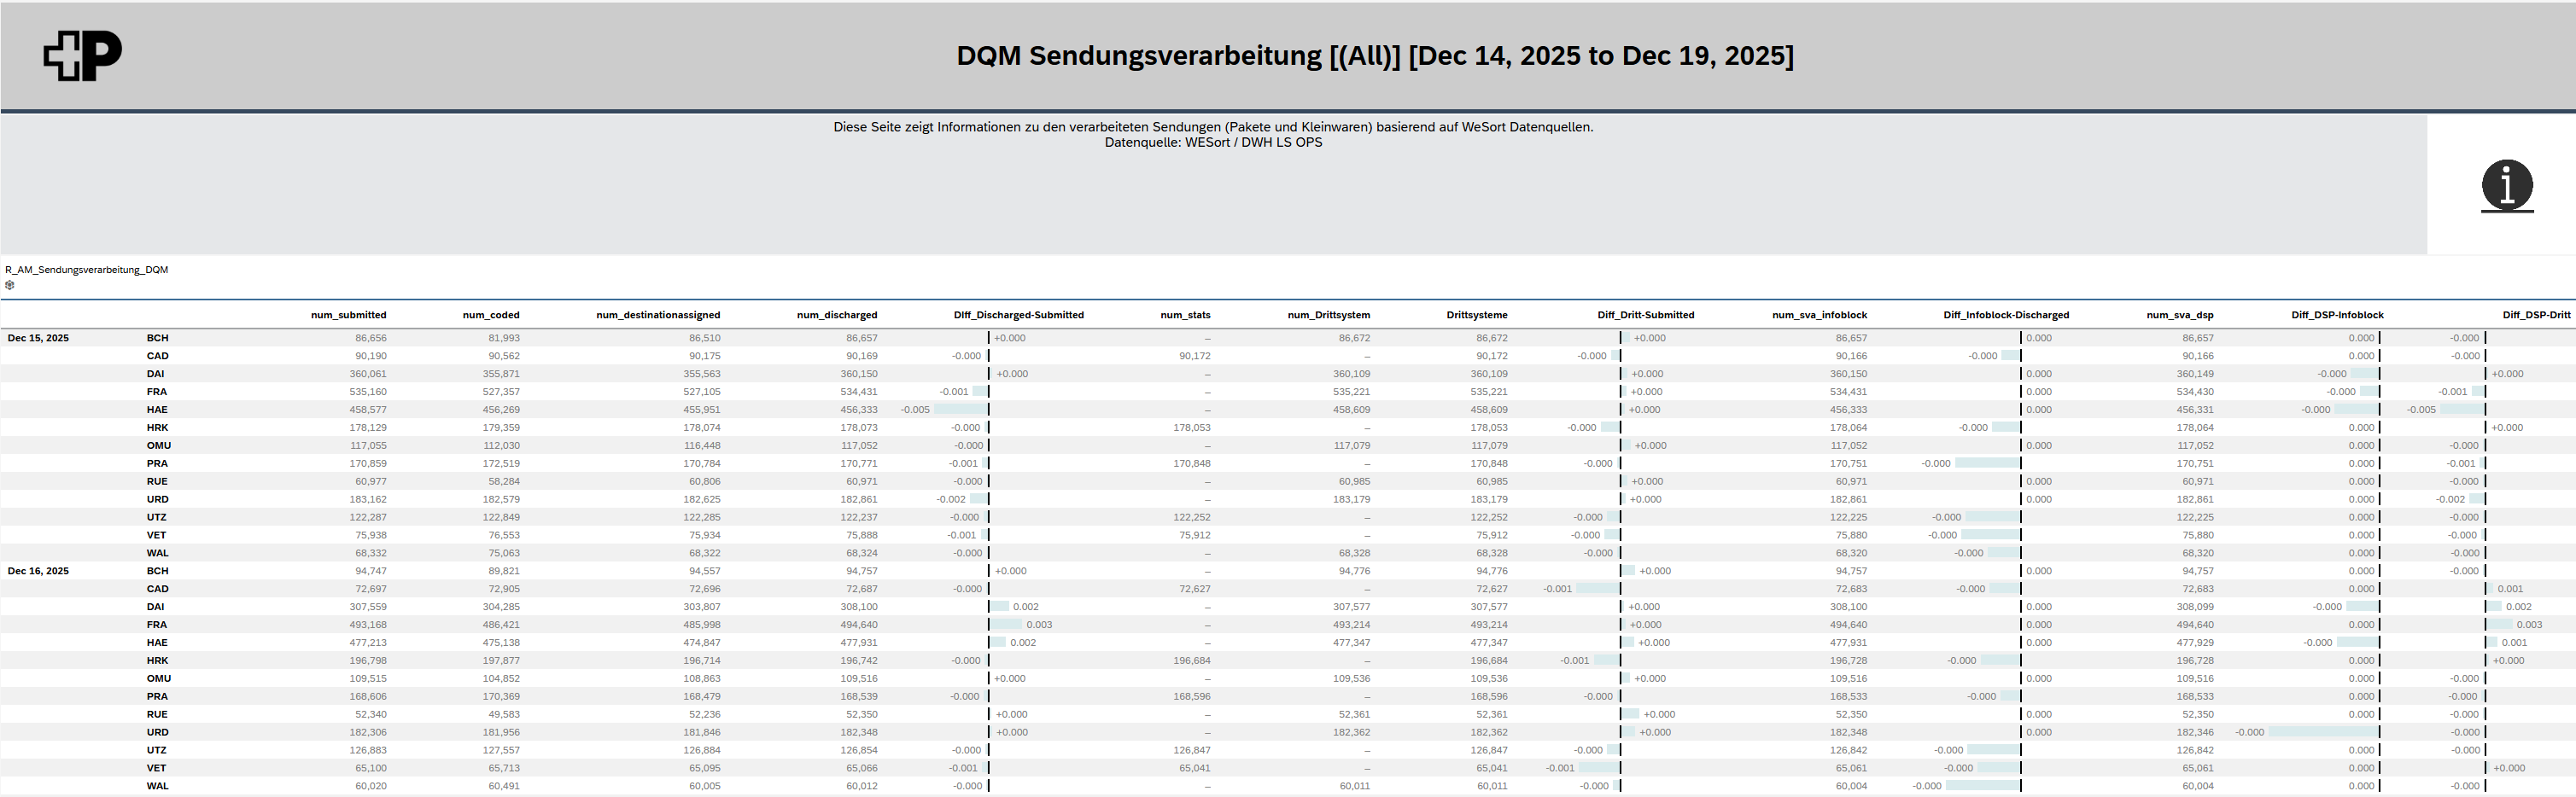
\includegraphics[width=0.95\textwidth]{./content/img/Plain_DQM_WEST_19-12-2025_08-43-34.png}
    \caption{Existing plain DQM dashboard used as the baseline for the redesigned Power BI report}
    \label{fig:plain_dqm_dashboard}
\end{figure}

To improve this situation, a report which hast to replace it, must be more visual. And apply some of the most basic business knowledge allowing to see its results faster. As the previous research has already defined which rules must be applied in an automatic check, those rules are the basis for the reports visualisation.

\subsubsection{Business stakeholder feedback}
During meetings with the business their requirements were accumulated. Those were simple, the report had to be upgraded to use the new data source. Since with the adoption of Power BI, also a more efficient reporting datastructure was possible, it had to be again measurable. As the data itself was only rearranged but not radically new, the checks and the way they had to be shown in a table stayed the same. Regarding additional improvements of the report no direction was given, however an OK was provided to improve the report with useful information.



\subsection*{DevOps}
At Swiss Post deployments are done by the software engineers effectively turning their field of operations to \gls{DevOps}. 

The field of DevOps is described by Wikipedia as follows \cite{enwiki:1362982395}:
DevOps is the integration and automation of software development and information technology operations. DevOps encompasses the tasks necessary for software development and can lead to both shortening development time and improving the development life cycle. According to American software architect Neal Ford, DevOps, particularly through continuous delivery, employs the "bring the pain forward" principle by tackling challenging tasks early, fostering automation, and enabling swift issue detection.

Although debated, DevOps is generally characterized by three key principles: shared ownership, workflow automation, and rapid feedback. From an academic perspective, Len Bass, Ingo Weber, and Liming Zhu—three computer science researchers from the CSIRO and the Software Engineering Institute—defined DevOps as "a set of practices intended to reduce the time between committing a change to a system and the change being placed into normal production, while ensuring high quality". However, the term is used in multiple contexts. At its most successful, DevOps is a combination of specific practices, culture change, and tools.



\subsubsection*{DevOps at Swiss Post}
At Swiss Post this the DevOps process is already defined and is not changed by this project, it will apply all defined tools and rules. To name the general rules:


\begin{itemize}
    \item GitHub is used as CodeRepository using SSO with post accounts
    \item The access to repositories is limited and managed by a permission system
    \item Separate repositories exist for development and productive environments
    \item Repositories are also separated by function, e.g. repositories for teraform \gls{IaC} or sql scripts for \gls{athena}
    \item Development is performed on branches
    \item To merge branches a pull request is required, this triggeres GitHub actions
    \item The Github actions are performing checks depending on repository and function
    \item To merge code on production environments a review by another developer is required in addition to successful Github actions
    \item In addition to this deployment pipeline, DevOPS engineer continue maintaining and support their code
\end{itemize}



\subsubsection*{Frontend deployment pipelines}

Regarding frontend reports a similar process is already defined and also applie, not adapted by this project.
When deploying front end reports using Power BI, the process is happening entirely on the microsoft environments.
\begin{itemize}
    \item Reports are initially created on Power BI desktop
    \item Development and testing happens on the desktop version first
    \item The report is deployed from Power BI desktop to Microsoft Fabric, development environment
    \item The code is checked in using git integration in Microsoft 
    \item The report is tested first in the development environment
    \item Then it is deployed trough the defined pipeline to test environment
    \item Stakeholders are performing tests on test environment
    \item After successful tests and eventual fixes the go for productive deployment is given
    \item Productive deployment is done again trough the deployment pipeline
\end{itemize}

The deployment pipeline is shown in the below figure, showing the selection of environments from which the 3 steps process starts.

\begin{figure}[H]
    \centering
    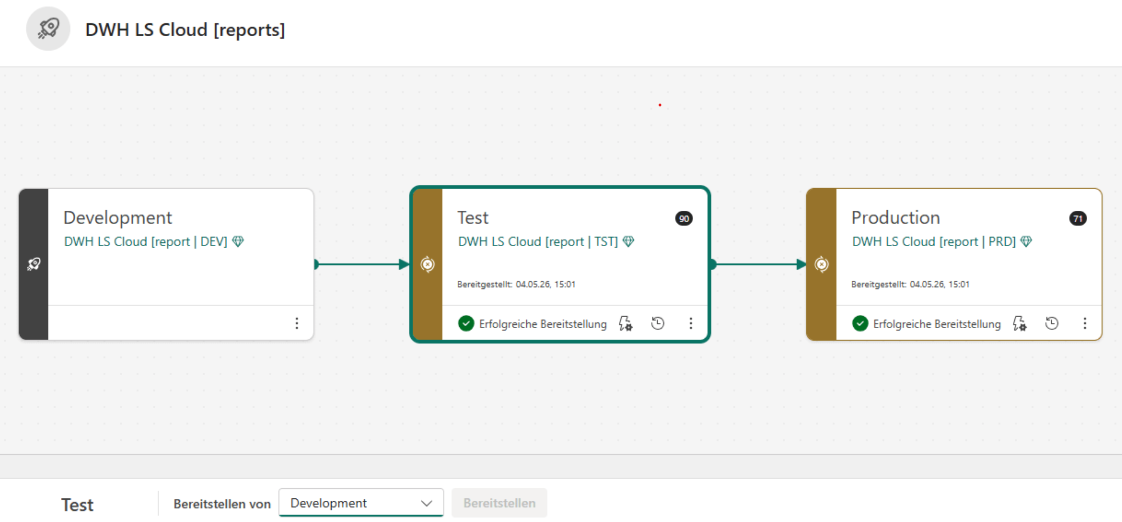
\includegraphics[width=0.95\textwidth]{./content/img/PowerBI_Deployment.png}
    \caption{Power BI deployment pipeline across the development, test, and production environments}
    \label{fig:powerbi_deployment_pipeline}
\end{figure}



\section{DQM tool selection}
The DQM tool selection required a structured approach. Such approach required to first setup a list of requirements towards a tools. Then a evaluation how well tools are fulfilling these requirements. And finally the invitation of the fulfilling providers to demos.

\subsection*{Tool selection principles}
the first step in evaluating a tool must be to get to know, what a tools actually needs to have. Commonly those lists are called requirement lists.
They have to incorporate the must have features of a tool and the nice to have requirements. With such a list, the decision together with higher management is made easier, as they allow for a scoring and easy overview of which tool scored how many points. Based on such points list, the per performing or best price can be selected.

\subsection*{Requirements list}
At Swiss Post the \gls{DQM} team setup the requirements list. It incorporates the following main principles:

\begin{itemize}
    \item \textbf{Data Coverage \& Connectivity:} The integration into the existing tool landscape. The requiements to be cloud first. Most important data sources that need to be handled.
    \item \textbf{Data Quality Capabilities:} What actual DQM requirements the tool must fullfill. The usability which is expected, such as NoCode environments.
    \item \textbf{Reporting \& Monitoring:} The tool must allow exports to other tools for reporting purpose.
    \item \textbf{Performance and Reliability:} The tool needs to be responsive also on big datasets as Swiss Post will want to run checks on very large transaction datasets.
    \item \textbf{Cost \& Licensing:} The cost of a tool is relevant. How is the cost structured.
\end{itemize}

\begin{figure}[H]
    \centering
    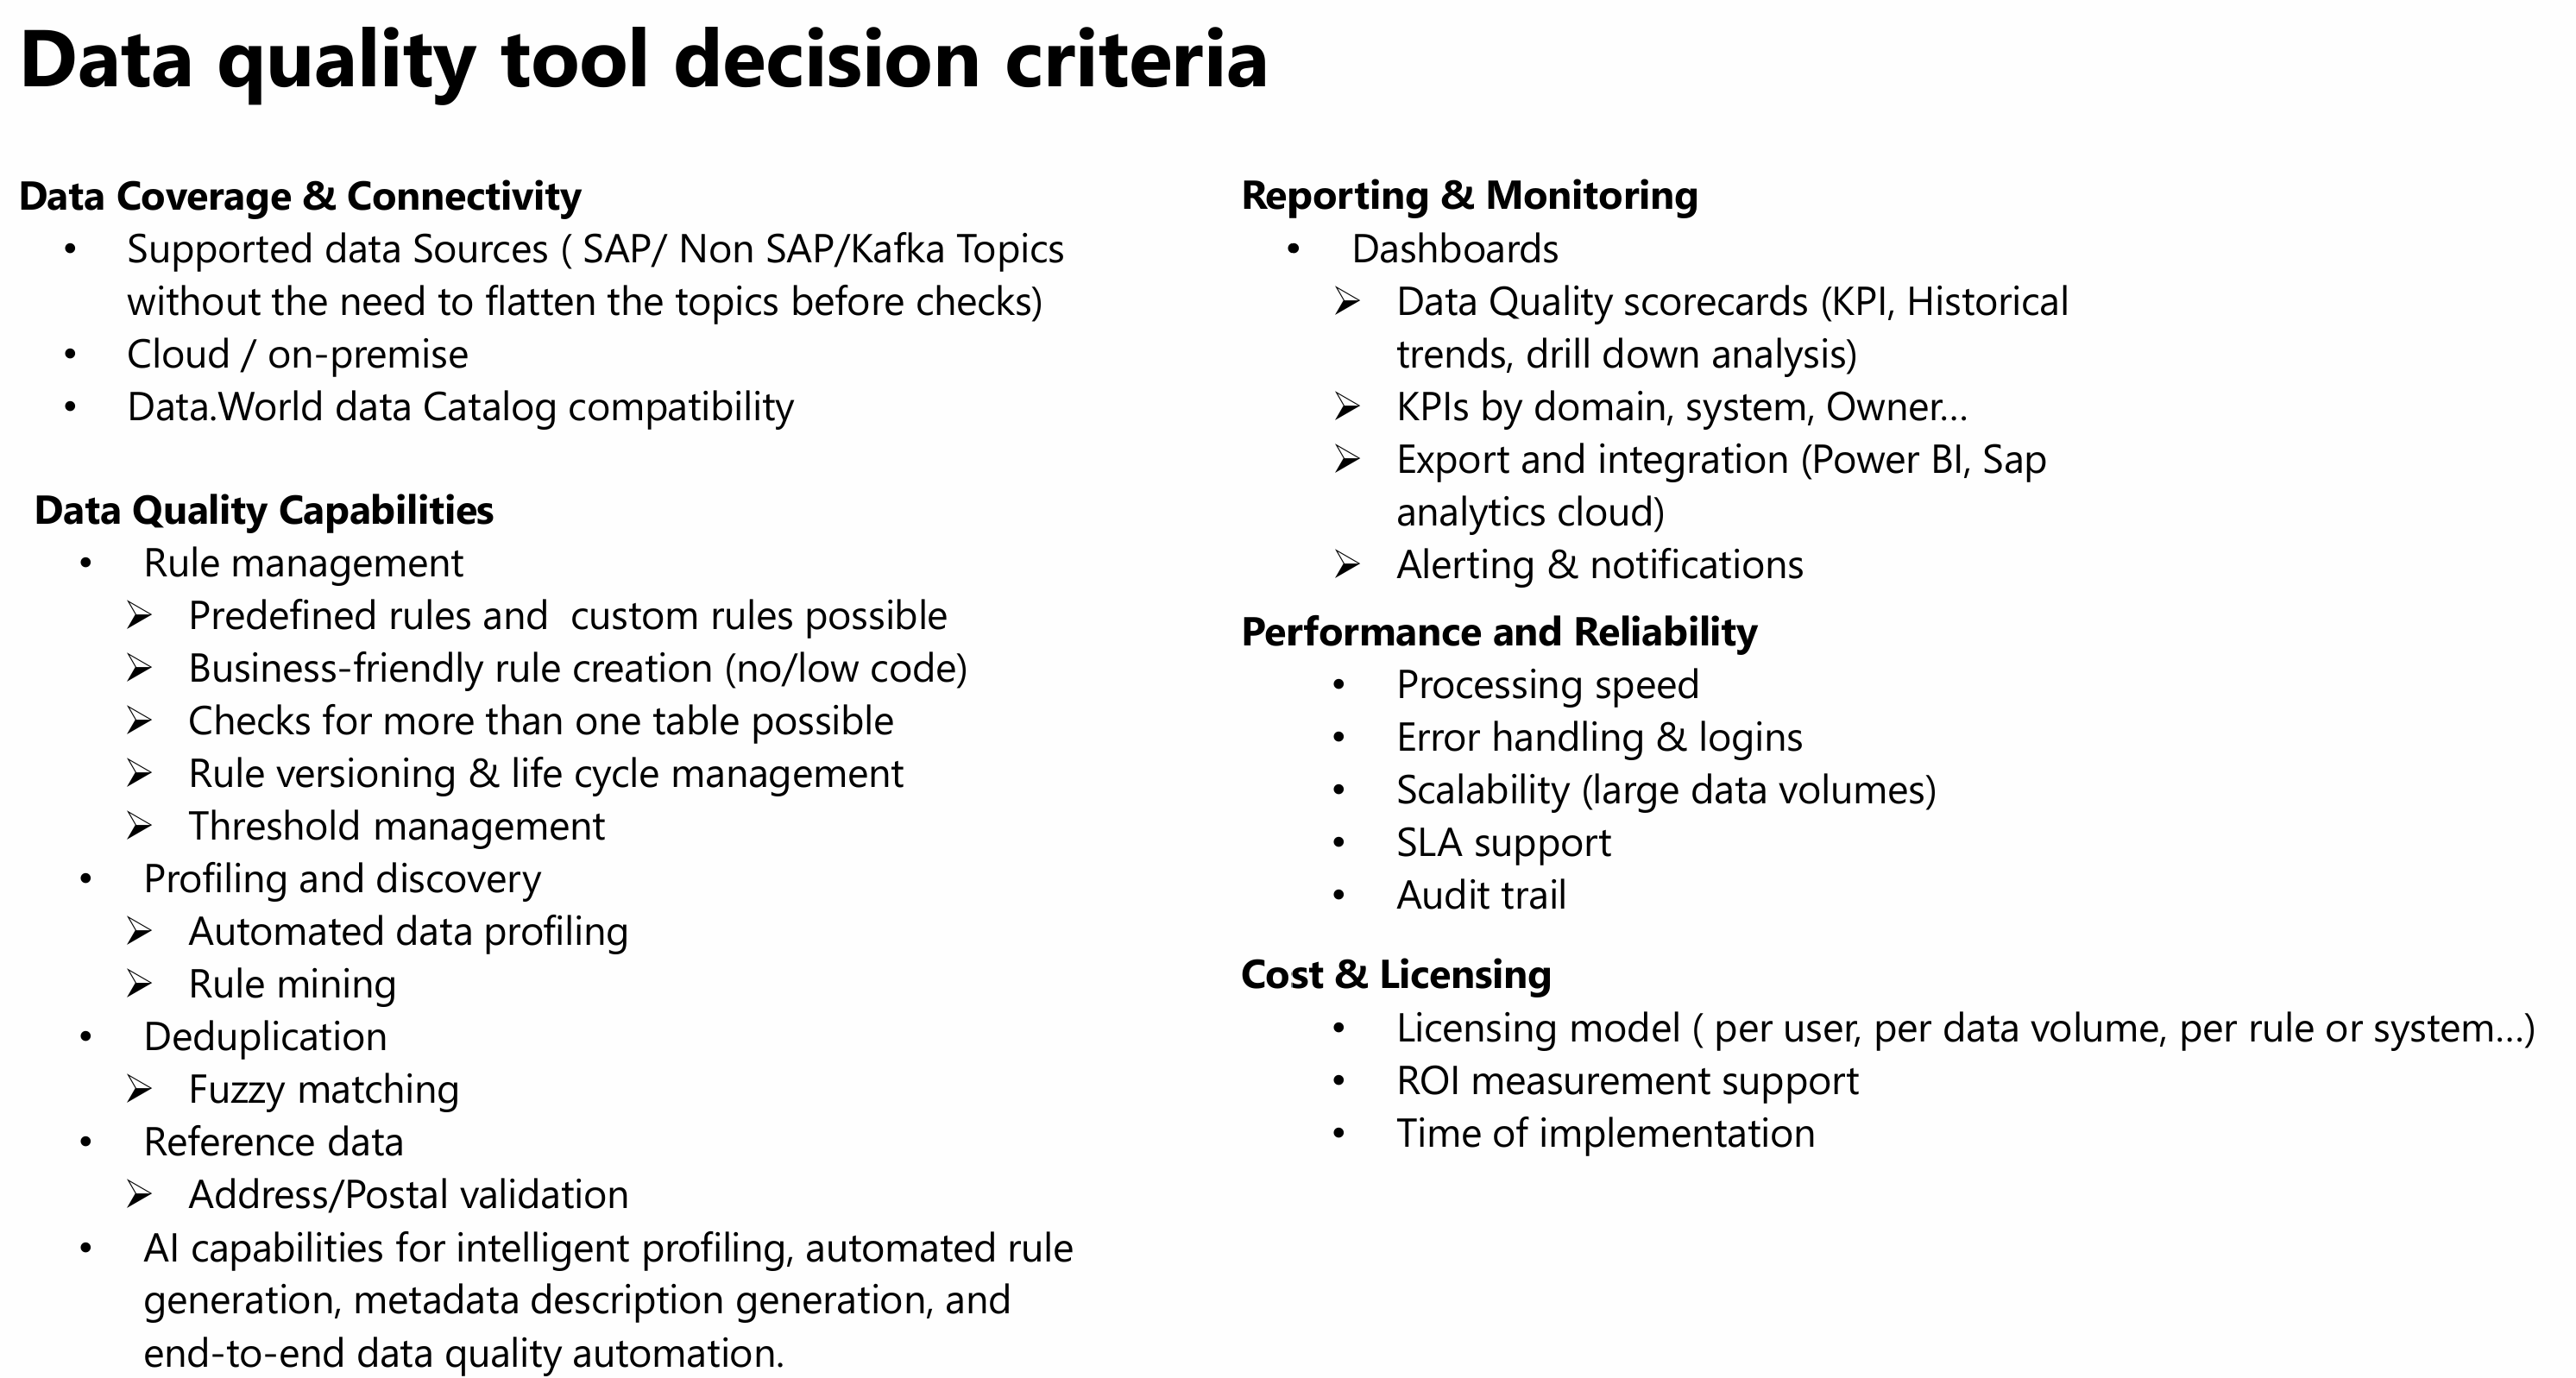
\includegraphics[width=0.95\textwidth]{./content/PostInput1/DQM_Tool_Evaluation_1.png}
    \caption{Overview of the data quality management tool evaluation process and the assessed evaluation criteria}
    \label{fig:dqm_tool_evaluation_1}
\end{figure}

Additionally there are the more \gls{softcriteria} which are nice to have. Soft criteria are the criteria which are not mandatory but make the usage of an application easier for users e.g. provide easy management of access roles. The list as defined by Swiss Post is shown in the following screenshot:

\begin{itemize}
    \item \textbf{Usability \& User experience:} User permission system allowing multiple different access levels and their provisioning trough existing means.
    \item \textbf{Technical requirements:} The security requirements which the cloud solution has to meet. Additionally the connectivity options they need to support
\end{itemize}

\begin{figure}[H]
    \centering
    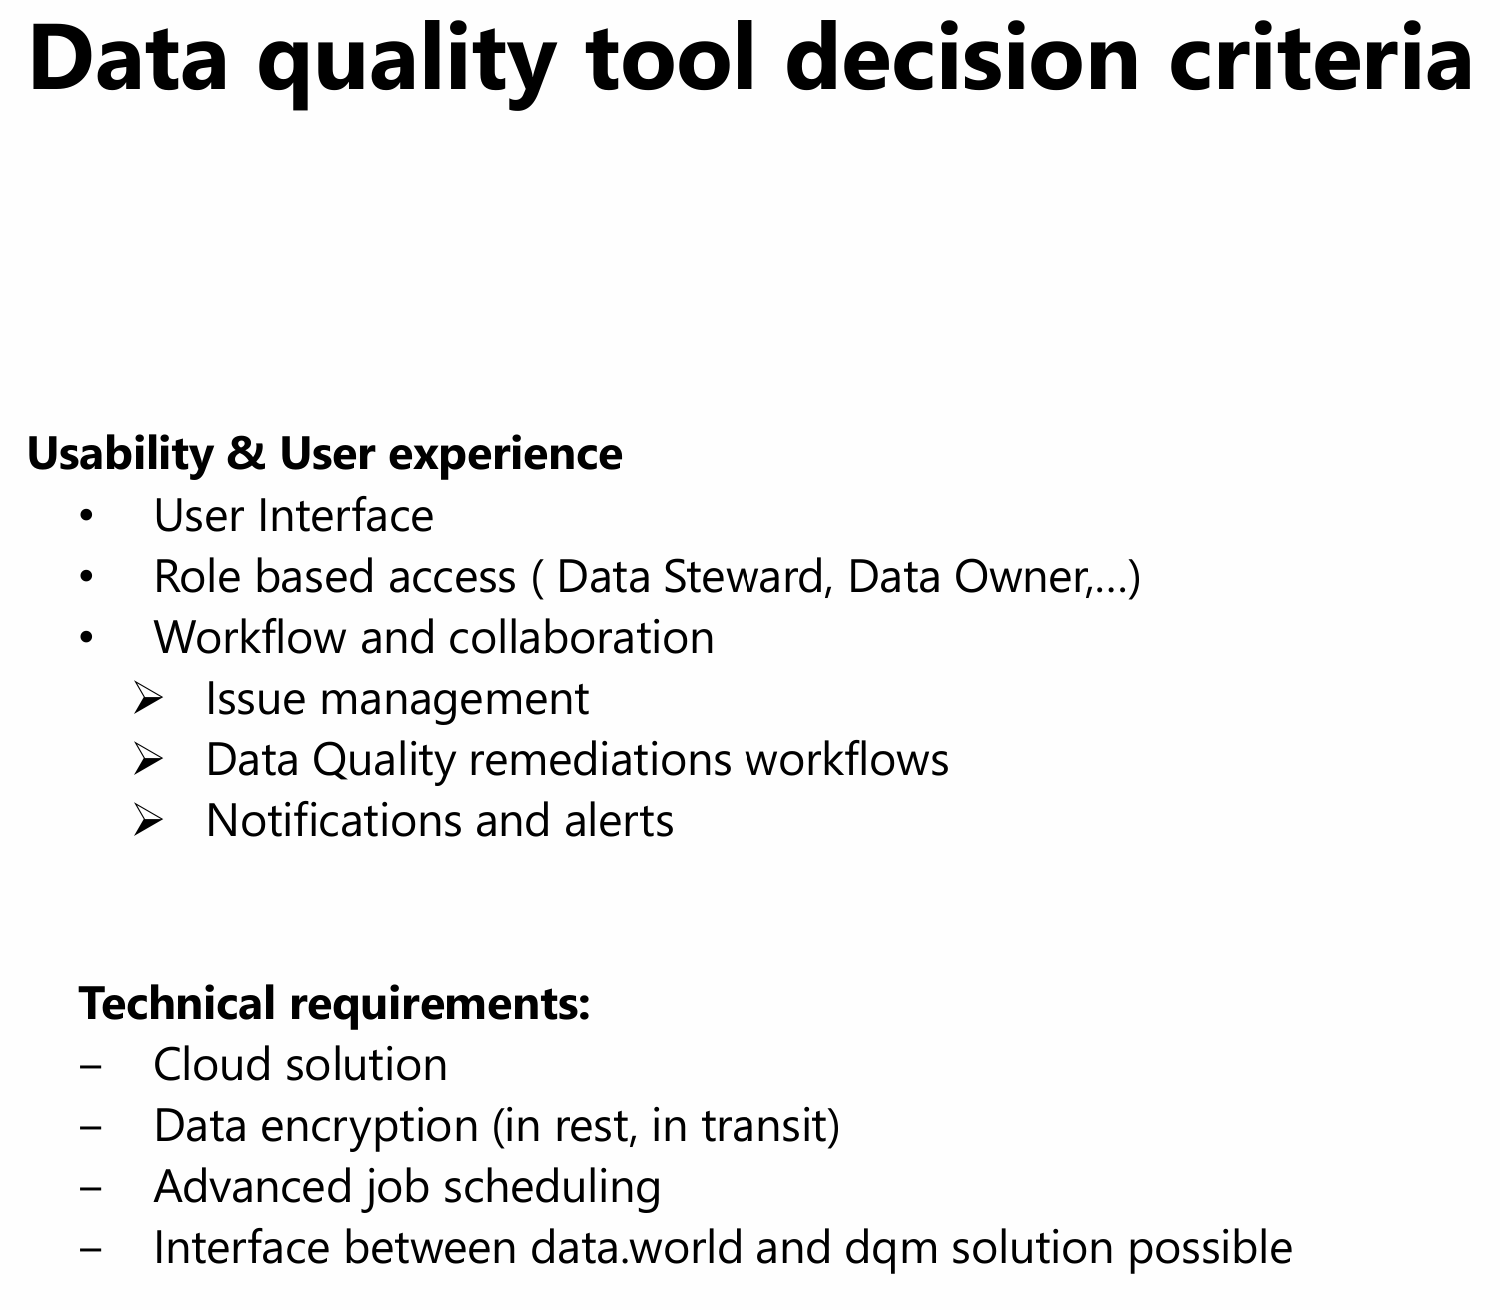
\includegraphics[width=0.45\textwidth]{./content/PostInput1/DQM_Tool_Evaluation_2.png}
    \caption{Continuation of the data quality management tool evaluation, including the comparison of the evaluated solutions}
    \label{fig:dqm_tool_evaluation_2}
\end{figure}

\subsection*{DQM tooling selection}
After having the selection criteria, the tools are researched. The research of these tools has also been done by the DQM team so its out of scope for this work.
As a result of the tool research, the different found tools are evaluated against the criteria. This finally results in the table as shown below highlighting the performance of the tools against criteria. This table the serves for which tools are inivited for demos or directly excluded. The following screenshots shows the five tools which made it into the evaluation, including the tree in green which were invited for demos.

\begin{itemize}
    \item \textbf{Ataccama ONE} : Selected for demo
    \item \textbf{Informatica IDMC (CDQ + optional Streaming)} : Selected for demo
    \item \textbf{Soda (Core + Cloud)} : Selected for demo. The demo is documented later in the document.
    \item \textbf{Great Expectations} : Not selected for demo
    \item \textbf{SAP Information Steward} : Not selected for demo
\end{itemize}


\begin{figure}[H]
    \centering
    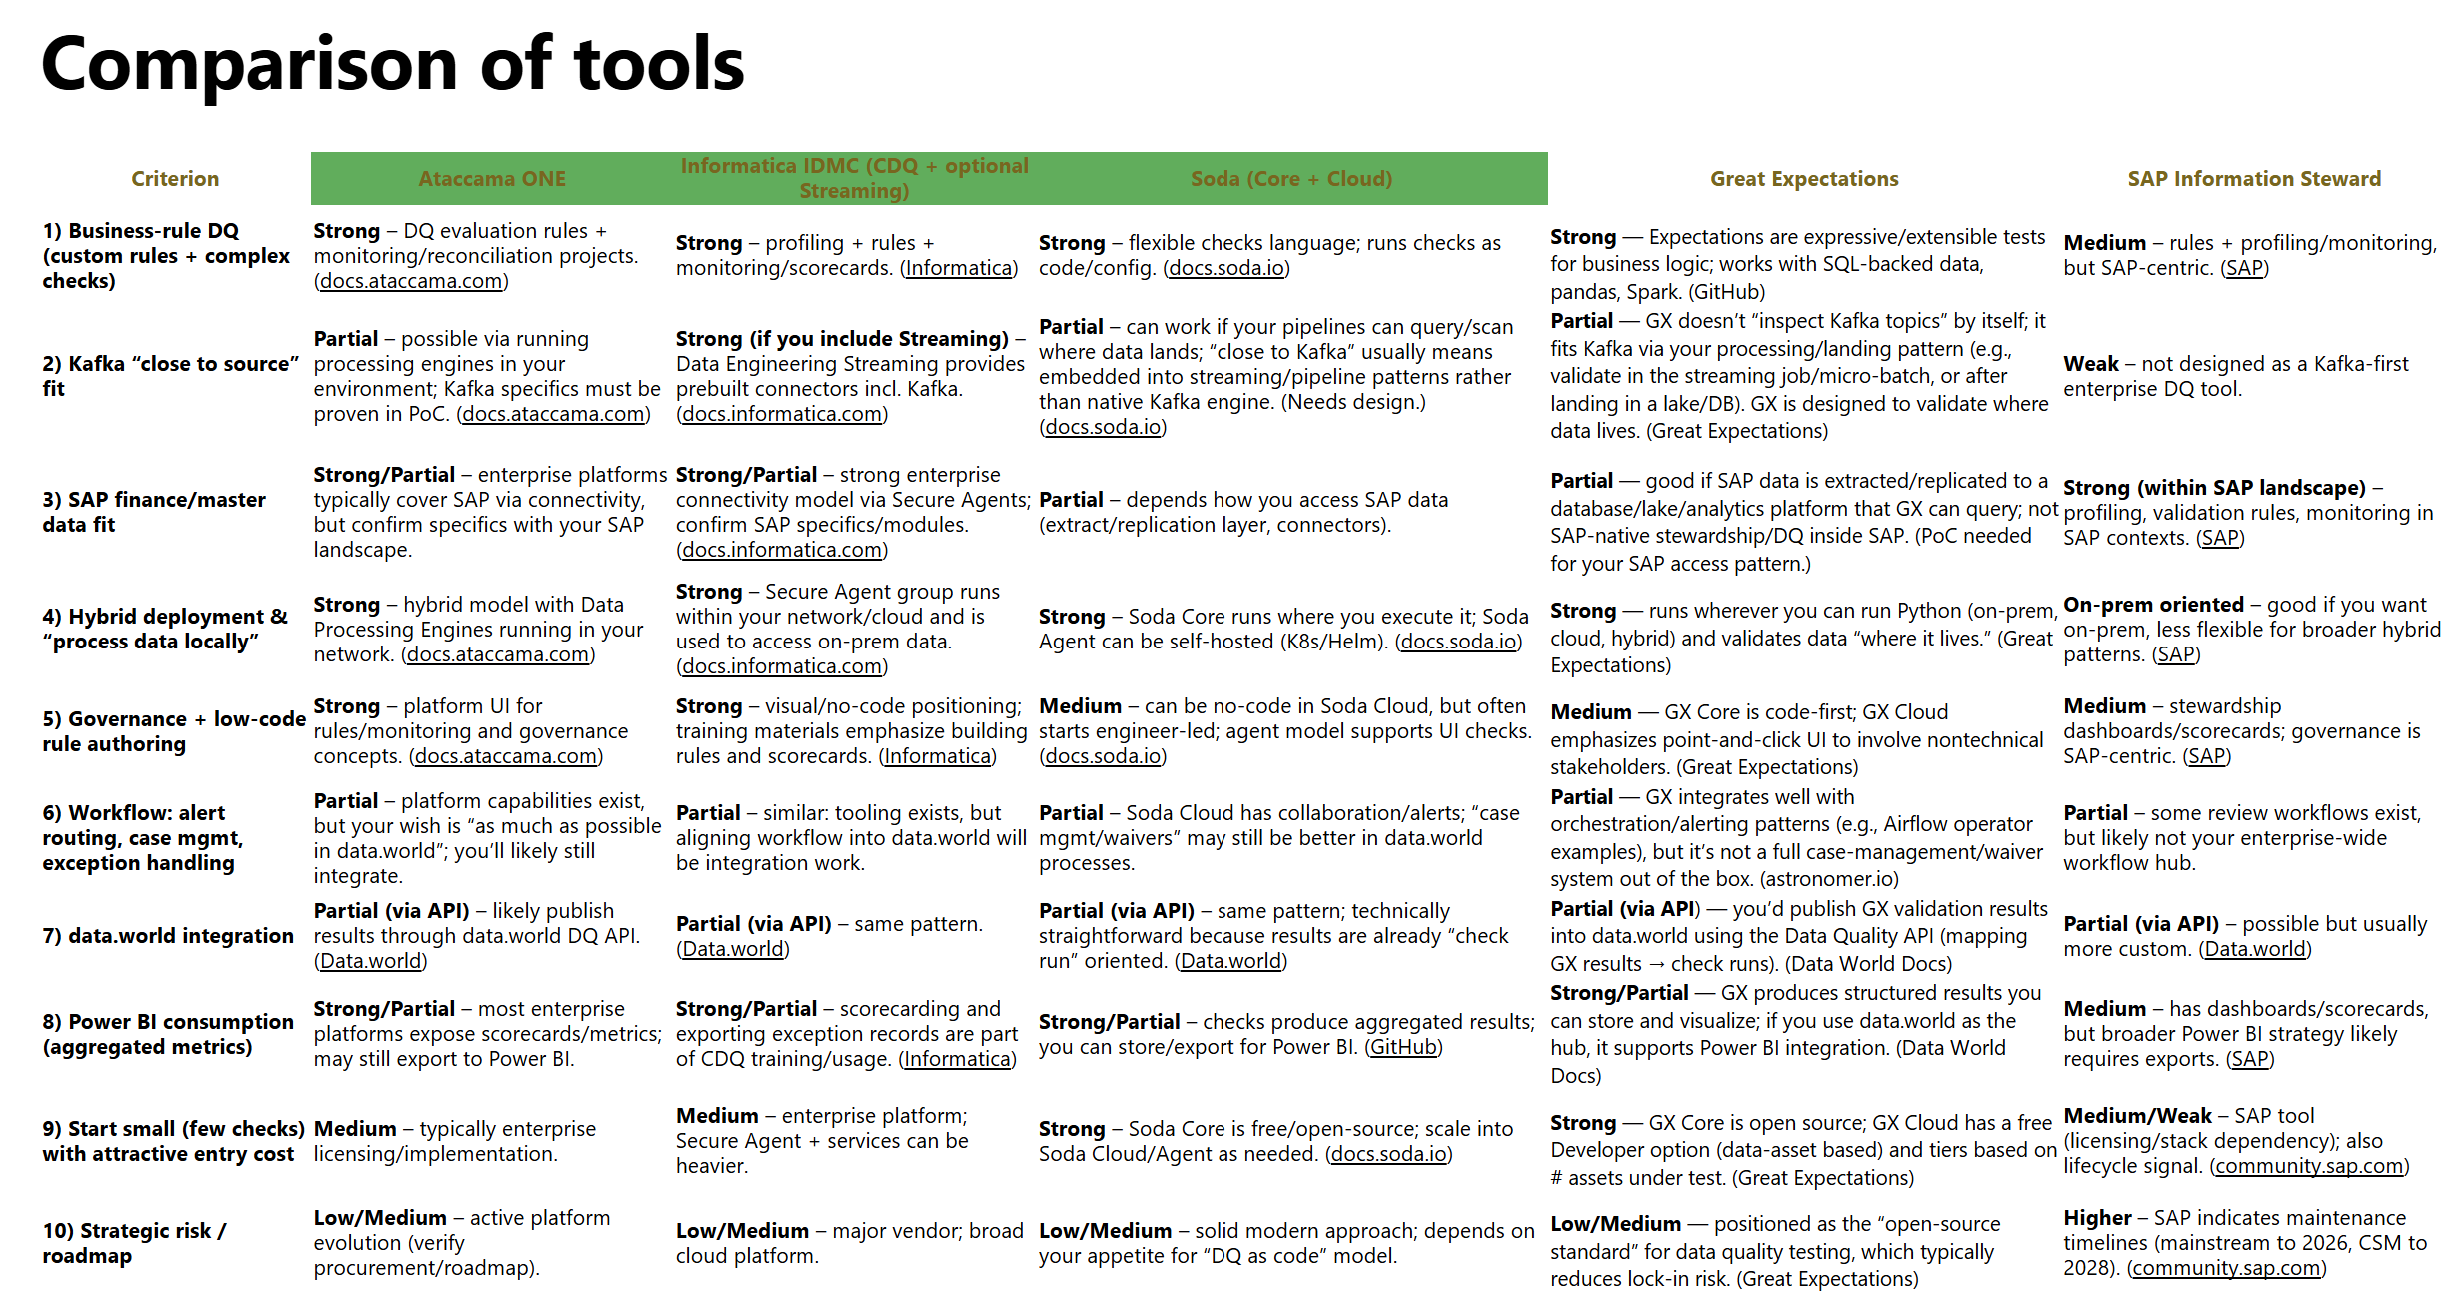
\includegraphics[width=0.95\textwidth]{./content/PostInput1/DQM_Tool_Evaluation_3.png}
    \caption{Example of the comparative evaluation matrix used during the assessment of different data quality management tools}
    \label{fig:dqm_tool_evaluation_3}
\end{figure}


\subsection*{Design decisions}
Next step after the evaluation table is to invite the succeeding tools to a demo. In this demo the providers are asked to show their performance of the tool against the defined criteria but can also show what specific benefit they bring with. The demo provides the selecting company with a more detailed view of the capabilities applied to their dataset or if any shortcommings are blocking the decision. Furthermore it allows the selecting company to directly ask questions on open items. After a demo the scoring can be adjusted and finally a decision made wether to go ahead with a provider into \gls{PoC} or even contract negotiations or send them the information that they dropped our of the selection.



\section{DQM tool testing}
Describes the testing of the tool...
what was required for an actual tool decision
What next follows
this is the basis for any work on the tool testing

\subsection*{Subsection No1}
This is the next subsection


